% !TEX encoding = UTF-8
% !TEX TS-program = pdflatex
% !TEX root = ../thesis.tex
% !TEX spellcheck = en_US

%************************************************
\chapter{Introduction}\label{chap:one}
%************************************************

General introductions

\section{The Standard Model of Particle Physics}
The standard model (\acs{SM}) of particle physics is a theory describing all known matter and their fundamental interactions except for gravity. It unifies the electromagnetic, weak, and strong forces under a single theoretical framework.
\begin{figure}
\centering
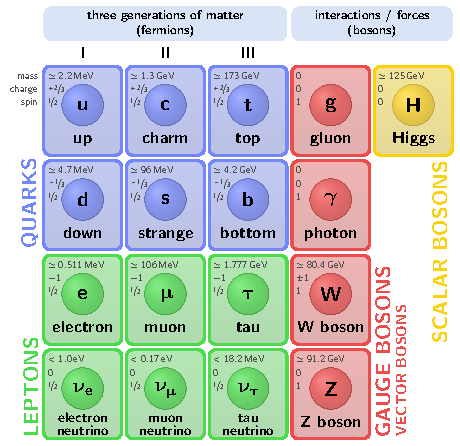
\includegraphics[width=0.7\textwidth]{Images/SM.pdf}
\caption{Elementary particles of the \acs{SM}. The was image generated with the help of Ref.~\cite{Neutelings_2024}.}
\label{fig:1:SM}
\end{figure}
The matter content of the \acs{SM} is classified into two primary groups: \textit{fermions} and \textit{bosons}. The fermions have spin $1/2$ and are further subcategorized into \textit{quarks} and \textit{leptons}. Quarks take part in the strong interactions, whereas leptons only interact via the electromagnetic or weak force. Bosons on the other hand have full integer spin. There exists a single particle with spin 0, the \textit{Higgs} boson, and four vector bosons, namely the gluon, the photon, and the $W$ and $Z$ boson. The vector bosons act as force carrier for the strong, the electromagnetic and the weak force respectively. The matter content of the \acs{SM} is also illustrated in Fig.~\ref{fig:1:SM}. The interactions between the particles are described by a non-abelian gauge theory of the $\SU{3}_C \times \SU{2}_L \times \U{1}_Y$ group which is spontaneously broken into $\SU{3}_C \times \U{1}_Q$, where the subscripts stand for \textit{color} ($C$), \textit{left-handed} ($L$), \textit{weak hypercharge} ($Y$) and \textit{electric charge} ($Q$). The quarks transform under the fundamental representation of $\SU{3}_C$, while the leptons do not interact strongly, \ie~they transform trivially under the same gauge symmetry. In the electroweak sector, the left-handed fermion fields form doublets which transform under the fundamental representation of the $\SU{2}_L$ group
\begin{equation}
\begin{gathered}
L_{iL} \equiv \begin{pmatrix}
\nu_{iL} \\
l_{iL}
\end{pmatrix}, \quad Q_{iL} \equiv \begin{pmatrix}
u_{iL} \\
d_{iL}
\end{pmatrix}, \\
\nu_i = \left( \nu_e, \nu_\mu, \nu_\tau \right),\quad  l_i = \left( e, \mu, \tau \right),\quad u_i = \left(u, c, t \right),\quad d_i = \left(d, s, b \right).
\end{gathered}
\end{equation}
After spontaneous symmetry breaking, we want to retain a non-chiral $\U{1}_Q$ gauge symmetry to represent the electromagnetic interactions. As a result, the particles must transform under the $\U{1}_Y$ gauge symmetry according to the \textit{Gell-Mann--Nishijima relation}:
\begin{equation}
\frac{Y}{2} = Q - I^3.
\end{equation}
With the particle charges displayed in Fig.~\ref{fig:1:SM} we then get
\begin{equation*}
\begin{tabular}{ccccccc}
  \hline
                & $L_{iL}$ & $Q_{iL}$ & $\nu_{iR}$ & $l_{iR}$ & $u_{iR}$ & $d_{iR}$ \\ \hline
  $\frac{Y}{2}$ & $-\frac{1}{2}$ & $\frac{1}{6}$ & $0$ & $-1$ & $\frac{2}{3}$ & $-\frac{1}{3}$ \\ \hline
\end{tabular}
\end{equation*}

The transformation properties of the gauge bosons is dictated by the covariance of the covariant derivative
\begin{equation}
\begin{gathered}
D_\mu \equiv \partial_\mu - i g A^a_\mu T_R^a - i g_2 W_\mu^a I^a + i g_Y \frac{Y}{2} B_\mu \\
T_R^a = \begin{cases} T^a \quad &\text{for quarks}, \\
  0 \quad &\text{for leptons},
\end{cases}
\qquad I^a = \begin{cases} \frac{\tau}{2} \quad &\text{for left-handed fermions}, \\
  0 \quad &\text{for right-handed fermions},
\end{cases}
\end{gathered}
\end{equation}
where $T^a$ and $\tau^a$ are the \textit{Gell-Mann} and \textit{Pauli} matrices.

Before spontaneous symmetry breaking, the Lagrangian which governs the evolution of all matter fields must be invariant under the $\SU{3}_C \times \SU{2}_L \times \U{1}_Y$ gauge group. Up to a \Charge\Parity\ violating term\footnote{The absence of the \Charge\Parity\ violating term $\theta \frac{g^2}{64 \pi^2}\epsilon^{\mu \nu \alpha \beta} F^{a}_{\mu \nu} F^{a}_{\alpha \beta}$ is an unsolved problem of particle physics, known as the strong CP problem.} the SM Lagrangian is the most general mass-dimension four Lagrangian for the described particle content
\begin{equation}
\mathcal{L}_\mathrm{SM} = \mathcal{L}_G + \mathcal{L}_F + \mathcal{L}_Y + \mathcal{L}_H.
\end{equation}
The gauge-field Lagrangian $\mathcal{L}_G$ describes the free propagation and in the case of the non-abelian groups $\SU{3}_C$ and $\SU{2}_L$ also the self-interaction of the gauge bosons. It is given by
\begin{equation}
\begin{gathered}
\mathcal{L}_G = - \frac{1}{4} G^{a}_{\mu \nu} G^{a\, \mu\nu} - \frac{1}{4} W^a_{\mu \nu} W^{a\, \mu\nu} - \frac{1}{4} B_{\mu\nu} B^{\mu \nu}, \\
G^a_{\mu\nu} \equiv \partial_\mu A^a_\nu - \partial_\nu A^a_\mu + g f^{abc} A^b_\mu A^c_\nu, \\
W^a_{\mu\nu} \equiv \partial_\mu W^a_\nu - \partial_\nu W^a_\mu + g_2 \epsilon^{abc} W^b_\mu W^c_\nu, \\
B_{\mu\nu} \equiv \partial_\mu B_\nu - \partial_\nu B_\mu.
\end{gathered}
\end{equation}
The propagation of the fermions and their interaction with the gauge bosons is described by
\begin{equation}
\mathcal{L}_F = \bar{L}_{iL} i \slashed{D} L_{iL} + \bar{\nu}_{iR} i \slashed{D} \nu_{iR} + \bar{l}_{iR} i \slashed{D} l_{iR} + \bar{Q}_{iL} i \slashed{D} Q_{iL} + \bar{u}_{iR} i \slashed{D} u_{iR} + \bar{d}_{iR} i \slashed{D} d_{iR}.
\end{equation}

The Higgs field is a doublet of the $\SU{2}_L$ group. We want the field to have a non-vanishing vacuum expectation value (\acs{VEV}) to dynamically generate the fermion and boson masses. Of course, the vacuum cannot carry an electric charge, which means that the Higgs field must be electrically neutral along the direction of \textit{spontaneous symmetry breaking} (\acs{SSB}). We choose this to be the second component of the doublet. With the Gell-Mann--Nishijima relation we can then deduce that hypercharge of the doublet must be $Y = +1$. The Higgs doublet field thus takes the form
\begin{equation}
\Phi = \begin{pmatrix}
  \phi^+ \\
  \phi^0
\end{pmatrix},
\end{equation}
where the superscript indicates the electic charge.

In order to generate a non-vanishing \acs{VEV}, the Higgs field must be in a potential with a global minimum away from zero. Hence, the only gauge invariant mass-dimension four Lagrangian we can construct is
\begin{equation}
\begin{gathered}
\mathcal{L}_H = \left( D_\mu \Phi \right)^\dagger \left( D^\mu \Phi \right) - V(\Phi) \\
V(\Phi) = \lambda (\Phi^\dagger \Phi )^2 - \mu^2 \Phi^\dagger \Phi, \quad \mu^2, \lambda > 0.
\end{gathered}
\end{equation}
The minimum of the Higgs potential $V$ is at
\begin{equation}
\Phi_0^\dagger \Phi_0 = \frac{\mu^2}{2 \lambda} \equiv \frac{v^2}{2} \neq 0.
\end{equation}
After (\acs{SSB}) we can expand the Higgs field around its minimum
\begin{equation}
\Phi = \begin{pmatrix}
  \phi^+ \\
  \frac{1}{\sqrt{2}} ( v + H + i \xi ).
\end{pmatrix}
\end{equation}
With this parametrization, the fields $\phi^\pm$ and $\xi$ can always be eliminated through a gauge transformation, they are therefore not physical (\textit{would-be Goldstone bosons}). The real scalar field $H$ is the famous Higgs boson. After inserting the expansion in the Higgs Lagrangian, the mass of the Higgs can be read-of from its square term
\begin{equation}
m_H = \sqrt{2} \mu.
\end{equation}

\acs{SSB} enables the generation of vector boson masses without breaking the gauge symmetry explicitly. If we insert the expanded Higgs field in the Higgs Lagrangian, we obtain terms of the form
\begin{equation}
\begin{split}
\mathcal{L}_H &\supsetneq \frac{v^2}{2} \bigg \lbrace g_2^2 \begin{pmatrix} 0 & 1 \end{pmatrix} I^a I^b \begin{pmatrix} 0 \\ 1 \end{pmatrix} W^a_\mu W^{b\, \mu} - g_2 g_Y \begin{pmatrix} 0 & 1 \end{pmatrix} I^a \begin{pmatrix} 0 \\ 1 \end{pmatrix} W_\mu^a B^\mu + \frac{g_Y^2}{4} B_\mu B^\mu \bigg \rbrace \\
&= \frac{v^2}{2} \bigg \lbrace \frac{g_2^2}{4} \left[ (W^1)^2 + (W^2)^2 \right] + \frac{1}{4} \begin{pmatrix} B^\mu & W^{3\, \mu} \end{pmatrix} \begin{pmatrix}  g_Y^2 & g_Y g_2 \\ g_Y g_2 & g_2^2 \end{pmatrix} \begin{pmatrix} B_\mu \\ W^3_\mu \end{pmatrix} \bigg \rbrace.
\end{split}
\end{equation}
By diagonalizing the mass matrix we obtain the physical states
\begin{equation}
\begin{gathered}
\begin{pmatrix}
A^\gamma_\mu \\
Z_\mu
\end{pmatrix} = \begin{pmatrix}
\cos \theta_W & - \sin \theta_W \\
\sin \theta_W & \cos \theta_W
\end{pmatrix} \begin{pmatrix}
B_\mu \\
W_\mu^3
\end{pmatrix}
\end{gathered}, \quad \cos \theta_W = \frac{g_2}{\sqrt{g_Y^2 + g_2^2}}, \sin \theta_W = \frac{g_Y}{\sqrt{g_Y^2 + g_2^2}}.
\end{equation}
In the new basis, we have one massless boson $A^\gamma_\mu$, which we identify as the photon and a charge neutral boson of mass
\begin{equation}
m_Z = \frac{v}{2} \sqrt{g_Y^2 + g_2^2}.
\end{equation}
The vector bosons $W^1$ and $W^2$ are not eigenstates of the charge operator. We therefore define the new states
\begin{equation}
W^\pm_\mu = \frac{1}{\sqrt{2}} \left( W^1_\mu \mp i W^2_\mu \right), \qquad Q W_\mu^\pm = \pm W_\mu^\pm,
\end{equation}
which are eigenstates of $Q$ and have mass
\begin{equation}
m_W = \frac{v}{2} g_2.
\end{equation}

Last but not least, we discuss the Yukawa sector of the \acs{SM} Lagrangian. Before \acs{SSB}, fermions cannot generate masses because a mass term would mix the left- and right-handed components of the fields, thereby breaking the chiral gauge symmetry. Here, once again, the Higgs field comes to the rescue: by coupling the fermions with the Higgs field through a Yukawa interaction\footnote{In the original formulation of the \acs{SM}, there are no neutrino Yukawa interactions, since they were believed to be massless. Neutrino oscillation experiments have shown however, that neutrinos do in fact have finite masses.}
\begin{equation}
\mathcal{L}_Y = - \left( y_{ij}^\nu \bar{L}_{iL} \Phi^c \nu_{jR} + y_{ij}^l \bar{L}_{iL} \Phi l_{jR} + y_{ij}^d \bar{Q}_{iL} \Phi d_{jR} + y_{ij}^u \bar{Q}_{iL} \Phi^c u_{jR} \right) + \hc,
\end{equation}
where $\Phi^c$ is the charge-conjugated field to $\Phi$, we do not explicitly break the symmetry. However, after \acs{SSB} this Lagrangian will generate exactly the required mixing between left- and right-handed fields to generate the fermion masses. The Yukawa-interaction matrices $y_{ij}^{\nu,l, d, u}$ can be shifted from the Yukawa sector to the fermion sector through a field redefinition. Indeed, if we apply the \textit{singular value decomposition} of the Yukawa matrix
\begin{equation}
y = U_L^\dagger y_{\mathrm{diag}} U_R, \quad \text{with} \quad (y_{\mathrm{diag}})_{ij} = m_i \delta_{ij}
\end{equation}
and redefine our fermion fields to be
\begin{equation}
f_{iR} \longrightarrow U_{Rij} f_{jR}, \qquad f_{iL} \longrightarrow U_{Lij} f_{jL}, \qquad f = \nu, l, u, d
\end{equation}
the Yukawa Lagrangian becomes
\begin{equation}
\mathcal{L}_Y = - \sum_{i}\left( m_{\nu_i} \bar{\nu}_i \nu_i + m_{l_i} \bar{l}_i l_i + m_{u_i} \bar{u}_i u_i + m_{d_i} \bar{d}_i d_i \right)  \left(1 + \frac{H}{v} \right).
\end{equation}
As an immediate consequence, we observe that the Yukawa coupling of the Higgs to the fermions is proportional to the mass of that fermion.
The field redefinition is a change from a flavor eigenbasis, which is diagonal in the couplings to the gauge bosons, to a mass eigenbasis. In the mass eigenbasis the part of fermion Lagrangian which contains the interaction to the electroweak gauge bosons after SSB is
\begin{equation}
\begin{split}
\mathcal{L}_F \supsetneq &\sum_f (-Q_f) e \bar{f}_i \slashed{A}^\gamma f_i + \sum_f \frac{e}{\sin \theta_W \cos \theta_W} \bar{f}_i ( I_f^3 \gamma^\mu P_L - \sin^2 \theta_W Q_f \gamma^\mu) f_i Z_\mu \\
&+ \frac{e}{\sqrt{2} \sin \theta_W} \left( \bar{u}_i \gamma^\mu P_L (V_\mathrm{CKM})_{ij} d_j W_\mu^+ + \bar{d}_i \gamma^\mu P_L (V_{\mathrm{CKM}}^\dagger)_{ij} u_j W_\mu^- \right) \\
&+ \frac{e}{\sqrt{2} \sin \theta_W} \left( \bar{\nu}_i \gamma^\mu P_L (V_\mathrm{PMNS}^\dagger)_{ij} l_j W_{\mu}^+ + \bar{l}_i \gamma^\mu P_L (V_\mathrm{PMNS})_{ij} v_j W_\mu^- \right).
\end{split}
\end{equation}
Here we identified the coupling constant
\begin{equation}
e = \frac{g_2 g_Y}{\sqrt{g_2^2 + g_Y^2}},
\end{equation}
as the factor in front of the photon interaction term. The \textit{CKM} and \textit{PMNS matrices}\footnote{Named after Cabibbo, Kobayashi and Maskawa, and Pontecorvo, Maki, Nakagawa and Sakata.} are the results of the field redefinitions
\begin{equation}
V_\mathrm{CKM} \equiv {U_L^{u}}^\dagger U_L^d, \qquad V_\mathrm{PMNS} \equiv {U_L^{l}}^\dagger U_L^\nu.
\end{equation}




\section{Higgs Production}
Here I explain why the Higgs production cross section is so important.

